\documentclass[a4paper, 11pt, oneside, openany, ngerman, onecolumn]{scrbook}

\usepackage[ngerman]{babel}
% Positionierung von Bildern
\usepackage{float}
% Bib
\usepackage{natbib}
% Tabelle formatieren
\usepackage{tabularx}
% Bilder einfügen
\usepackage{graphicx}
% URLs, Zeilenumbruch auch bei Bindestrichen
\PassOptionsToPackage{hyphens}{url}\usepackage[pdfencoding=unicode]{hyperref}
% Rechtschreibprüfung
\usepackage{spelling} 
% Quellcode einbinden
\usepackage{listings}
% Farben
\usepackage[table]{xcolor}
% TODO-Marker
\usepackage{todonotes}
% Subfigures
\usepackage{subcaption}
% Math
\usepackage{mathtools}
% Für Header
\usepackage{fancyhdr}
\pagestyle{fancy}
\fancypagestyle{plain}{}
% Header
\rhead{Sirk Petzold}
\lhead{\today}
\chead{tj18b}
\renewcommand{\headrulewidth}{0pt}
% Foot
\renewcommand{\footrulewidth}{0pt}

\renewcommand{\clearpage}{}
\vspace{\baselineskip}

\definecolor{stringcolor}{RGB}{0,150,20}
\definecolor{keywordcolor}{RGB}{0,90,230}
\definecolor{commentcolor}{RGB}{192,32,32}

\setlength{\parindent}{0em}
\setlength{\parskip}{1em}
\setlength{\extrarowheight}{5pt}

\begin{document}
\sloppy

\frontmatter
\begin{titlepage}
	\begin{center}
		{\Huge\textbf{Qualitätssicherungskonzept}\vspace{2em}}

		{\Large\textbf{Synchronisation und Auswertung von Roboterfußballvideos}\vspace{1em}}

		{\textsf{tj18b}\vspace{2em}}

		\begin{table}[b]
			\begin{tabularx}{\textwidth}{lXr}
				\textbf{Mitglieder}&&\textbf{Betreuer}\\
				Dan Häßler&&Hans-Gert Gräbe\\
				Robert Wagner&&Tobias Wieprich\\
				Sirk Petzold&&Tobias Jagla\\
				Alex Eichhorn&&André Köhler\\
				Erik Diener&&\\
				Jonas Wrubel&&\\
				Tomas Daetz Chacon&&\\
			\end{tabularx}
		\end{table}
	\end{center}
\end{titlepage}

\tableofcontents


\mainmatter
\newpage
\chapter{Visionen und Ziele}
\textbf{/LV10/} Das System soll für das NAO-Team HTWK die Bearbeitung und Auswertung von Videos einzelner Roboterfußballspiele vereinfachen und diverse Bearbeitungsmöglichkeiten bereitstellen.

\textbf{/LZ10/} Das System soll bis zu vier Videos mit festem Dateiformat und festgelegter FPS-Zahl und die dazugehörigen Logs automatisch synchronisieren. Dabei sollen möglichst viele Schritte editierbar und transparent gehalten werden.

\newpage
\chapter{Rahmenbedingungen und Produktübersicht}

Die Applikation gliedert sich aktuell in 5 wesentliche Bereiche.
Als zentrale Einheit dient die \textbf{Video-Area}, in der alle geladenen Videos abgespielt und alle Operationen abgebildet werden.

Die \textbf{Kontrolleinheit} enthält den Play-Button zum Abspielen der Videos, eine Stop und Skip-Funktion für 1 Frame, sowie eine Skip-Funktion für eine einstellbare Anzahl von Fames. Die Skipfunktionen wurden jeweils vorwärts und rückwärts implementiert. Deren Frameweite ist aktuell über die Einsetllungen bestimmt. Es gibt zusätzlich ein Drag\&Drop Funktion für Videos/Bilder und die globale Zeit von den Videos wird angezeigt. 

In der \textbf{Track-Area} werden die einzelnen Spuren für die Videos dargestellt, in denen entsprechende Markierungen gesetzt werden können die in der Speicherung im MLT-Format berücksichtigt werden. Die Spuren sind untereinander responsive und erlauben keine Überlappungen. Vom Nutzer erzeugte Überschneidungen werden demnach vom Programm automatisch korrigiert.

Die \textbf{Log-Area} dient der Darstellung der geparsesn Logfiles und selektiert stets das Element das zur aktuellen Videoposition passt. Darüber hinaus kann hier per Klick ein Element ausgewählt werden, wodurch alle Videos zu der entsprechenden Stelle gespult werden.

In der \textbf{Menüleiste} ist bereit das Öffnen und Speichern von MLT Dateien möglich. Man kann auch Videos, Bilder und Logs importieren. Von hier können auch die Einstellungen des Programm gesteuert werden.. 

Damit Komponenten die sich nicht aneinander gekoppelt sind sauber miteinander kommunizieren können, wurde ein Publish-Subscribe System in Form eines Eventbus implementiert. Dieser könnte allerdings noch durch den Einsatz einer Library ersetzt werden.
Die Anwendung ist in ihrer Größe dynamisch veränderlich, läuft aktuell unter Windows, Linux und MacOS und wird im Laufe der Entwicklung noch einige Verbesserungen bezüglich der Benutzeroberfläche erhalten. 
Die Darstellung der Videos wird in einem Anwenderfreundlicheren Kontext erweitert. Abdockbare Fenster sind hierbei aktuell im Gespräch.

\newpage
\chapter{Grundsätzliche Struktur- und Entwurfsprinzipien}

\section{Programmiersprachen/Markup}
Die ausschließlich verwendete Programmiersprache ist Java. FXML wird als markup language für das UI verwendet.

\section{Architektur/Struktur}
Die Software kommt ohne eine Server-Anwendung aus und ist eigenständig als Stand-Alone Application funktional.
Als Build-Tool wird Maven verwendet.

\section{Frameworks/Libraries}
Die grafische Benutzeroberfläche wird mit JavaFX und dem internen Tool SceneBuilder modelliert.
Da aber JavaFX im Bereich Audio- und Videomanipulation einigen unserer Anforderungen nicht gerecht wird, binden wir das Java Library openpnp (Java Bindung für OpenCV).

\section{Vorgehensweise}
Zuerst wurde ein Grundgerüst erstellt, welches bereits alle bisher für notwenig erachteten Klassen enthält und in dem der Großteil der geplanten Methoden deklariert ist (siehe Abschnitt \glqq Datenmodell\grqq).
Die einzelnen Funktionalitäten werden nacheinander - wie im Releaseplan beschrieben - entwickelt und zusammengeführt.
Leichte Abweichungen aufgrund von schwer vorhersehbaren Problemen waren eingeplant und sind bereits eingetreten. Darüber hinaus konnte bereits ein Vorsprung im Entwicklungsfortschritt gegenüber der Planung erwirkt werden. Dieser soll möglichst beibehalten werden, um ein Zeitfenster zur Lösung eventuell größerer Probleme zu gewährleisten.
\newpage
\chapter{Struktur- und Entwurfsprinzipien einzelner Pakete}

\section{Package: Source Packages}
Dieses Package beinhaltet die entwickelten Java Module, welche sich aus java Dateien zusammensetzen. Dabei ist weitestgehend jedes Package als Modul implementiert.

\begin{tabularx}{\textwidth}{lX}
\textbf{robokicker.config}&Parameter/Konfigurierbare Werte\\
\textbf{robokicker.pubsub}&EventBus Implementierung des Publish-Subscribe Pattern\\
\textbf{robokicker.log}&Log file parse, LogPane als GUI-Controller zur zugehörigen FXML, Log Entry als Datenstruktur\\
\textbf{robokicker.menu}&Menu, SettingsMenu als GUI-Controller\\
\textbf{robokicker.track}&TrackRange als Datenstruktur, TrackPane als GUI-Controller und die TrackBox als Spurelement\\
\textbf{robokicker.scene}&Robokicker als main class, sowie Szene als GUI-Controller\\
\textbf{robokicker.videoplayer}&VideoPlayer, VideoPane als GUI-Controller\\
\textbf{robokicker.util}&Unterschiedliche Funktionalitäten\\
\textbf{robokicker.mltparser}&MLTReader für das Lesen von MLT Dateien, MLTTWriter für das schreiben MLT Dateien sowie unterschiedliche Datenstrukturen\\
\end{tabularx}

\section{Package: Test Packages}
Gleicher Aufbau wie source packages. Beinhaltet JUnit Tests zu jeder testrelevanten Klasse.

\section{Package: Resources}
In diesem Package liegen folgende hierarchisch untergeordneten Packages:

\begin{description}
	\item [fxml] Hier liegen alle FXML-Dateien, die die hierarchische Struktur und das Layout des GUI beschreiben. Dabei besitzt jede größere Komponente eine eigene fxml-Datei. Das macht den Code übersichtlicher und bringt dadurch Vorteile in der Wartbarkeit und Wiederverwendbarkeit.
	\item [help] In diesem Package liegen fast ausschließlich HTML-Dateien, die das Skript für das Help Menu bilden.
	\item [icons] In diesem Package liegen Icons.
	\item [styles] In diesem Package liegt die CSS Datei für das GUI.
	\item [test] In diesem Package liegen Videodateien und Textdateien zum Testen während des Entwickelns.
\end{description}
\chapter{Datenmodell}
\section{Config}
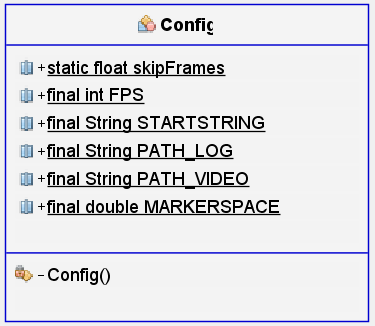
\includegraphics[scale=0.6]{configUML}
\section{Menu}
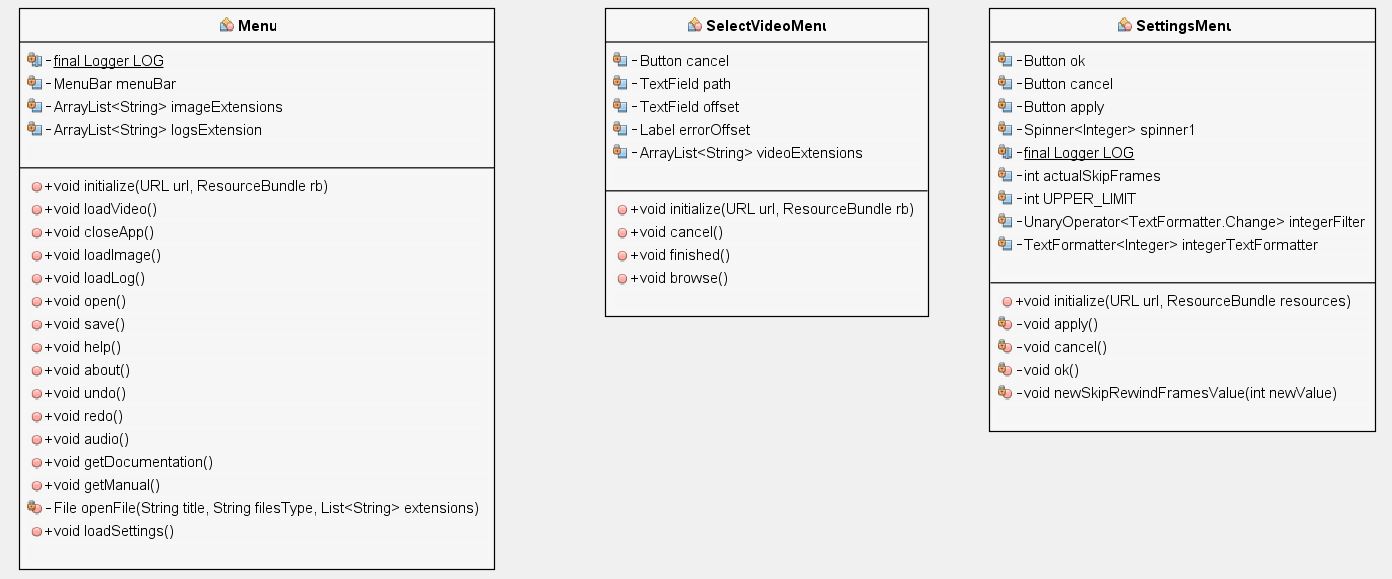
\includegraphics[scale=0.45]{menuUML}
\section{Trackpane}
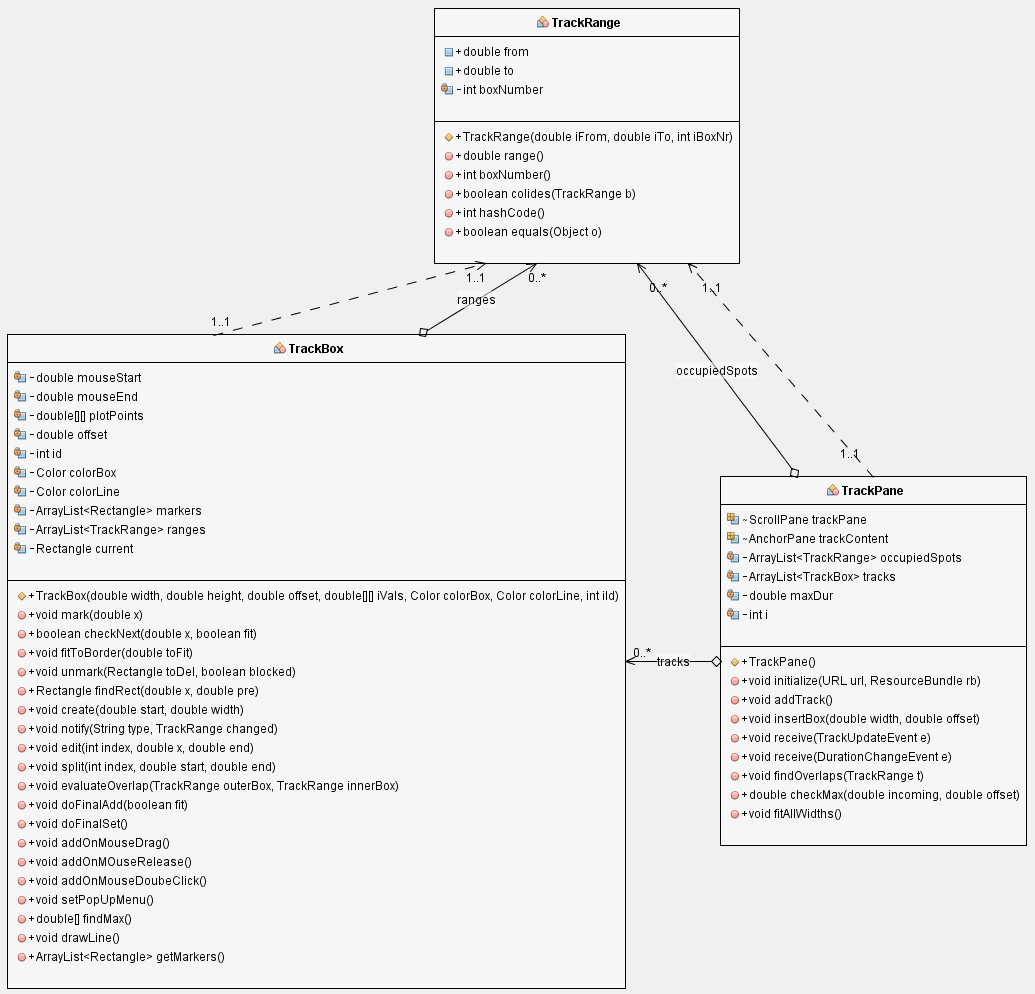
\includegraphics[scale=0.55]{trackUML}
\section{Logpane}
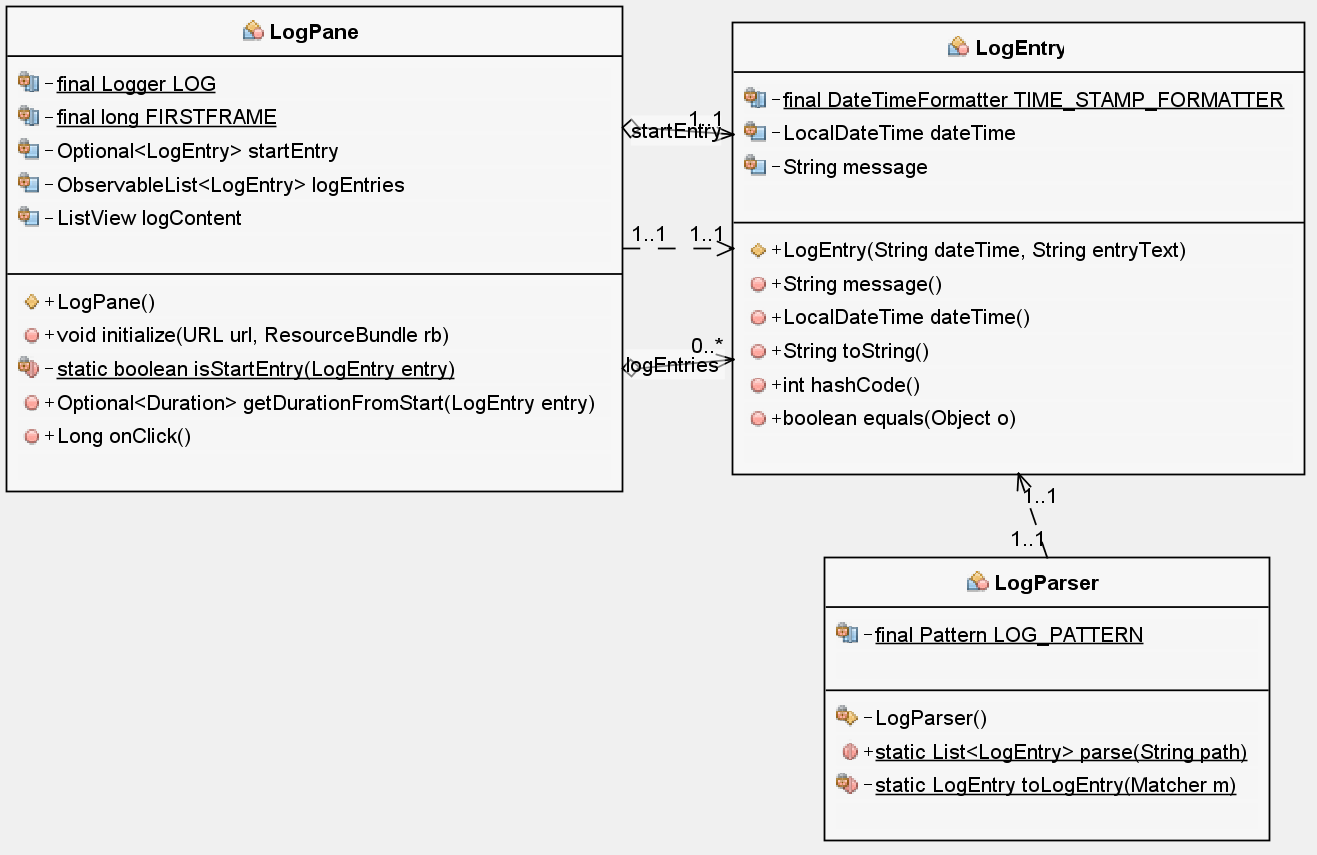
\includegraphics[scale=0.4]{logUML}
\section{Videopane}
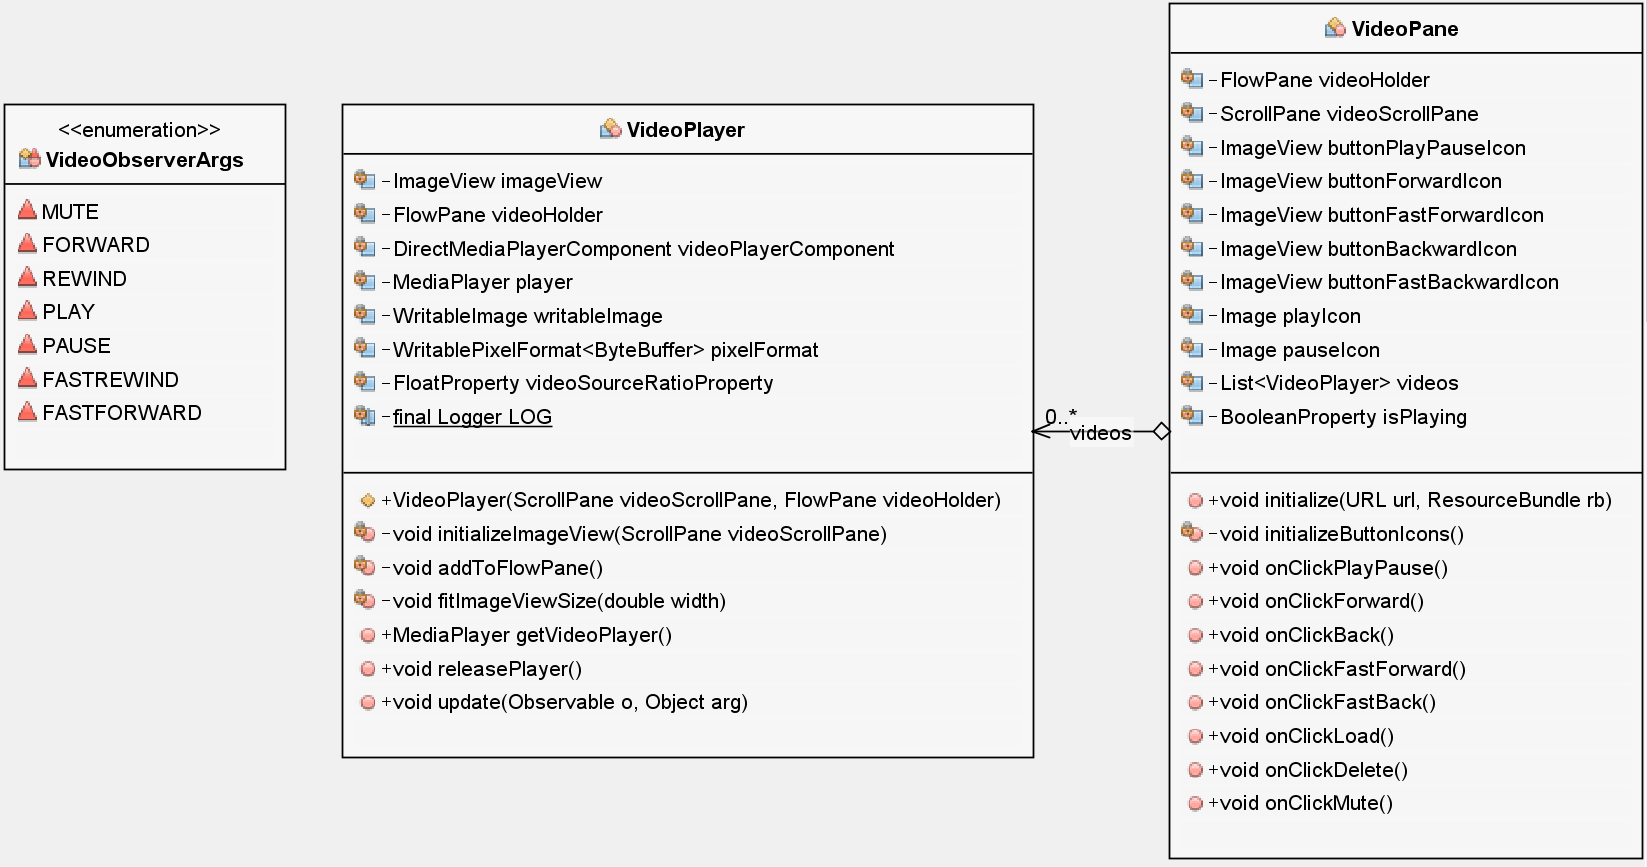
\includegraphics[scale=0.3]{videoUML}
\section{Eventbus}
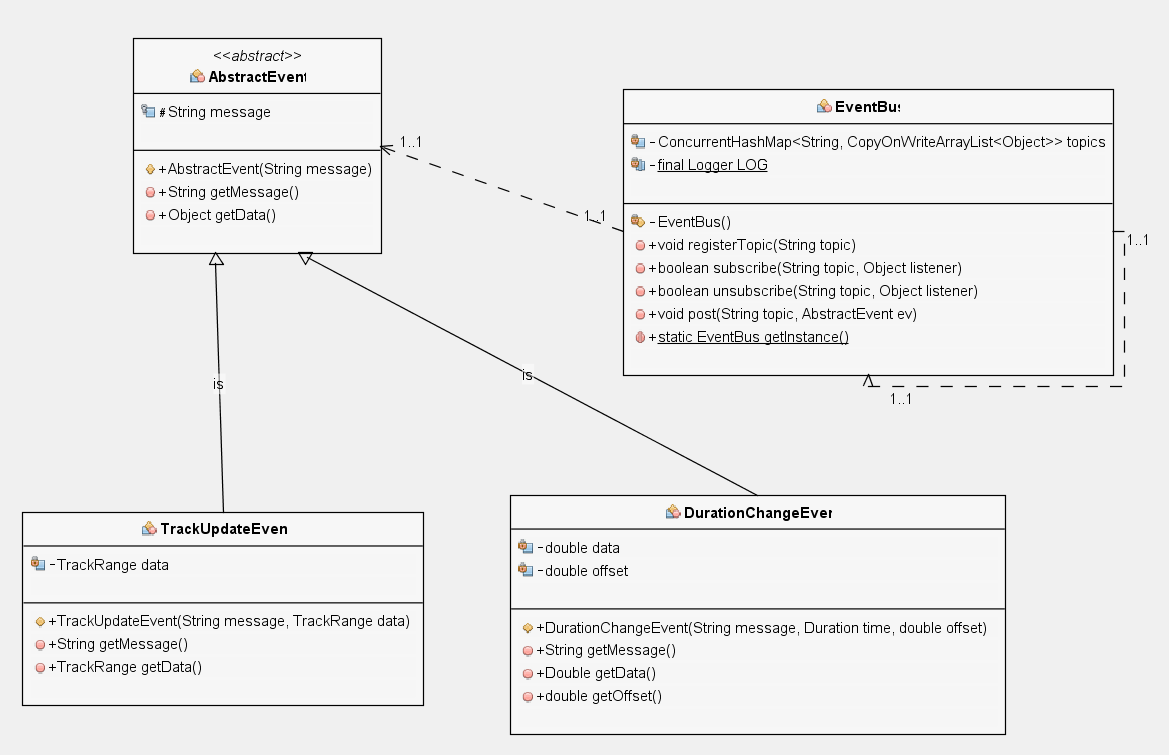
\includegraphics[scale=0.5]{eventUML}
\chapter{Publish-subscribe}
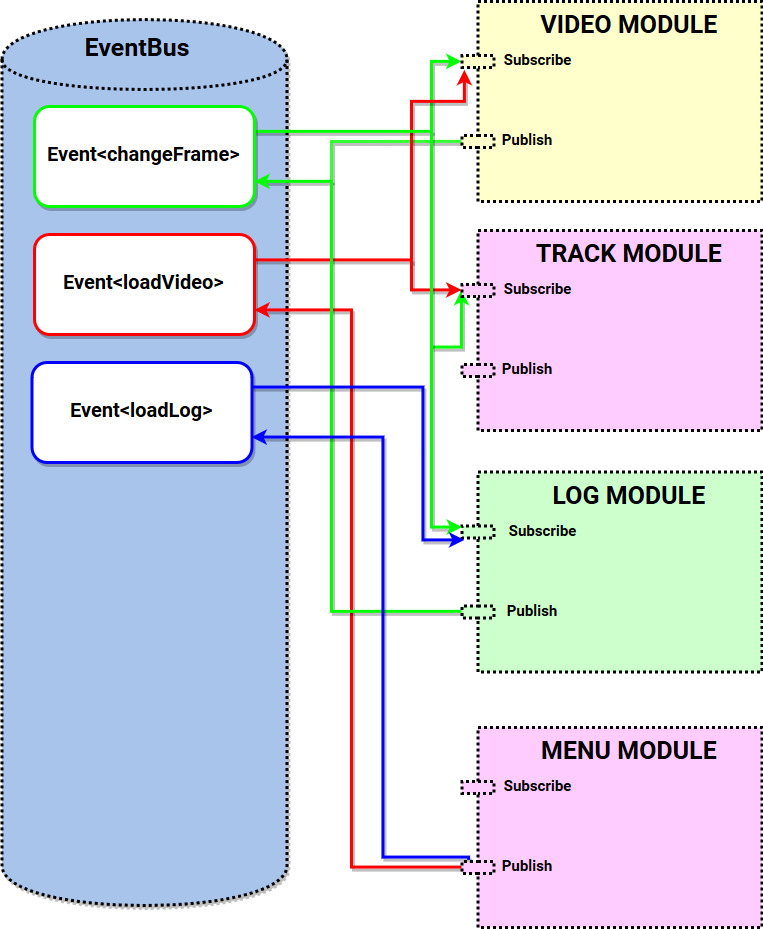
\includegraphics[scale=0.5]{eventbus}
\newpage
\chapter{Glossar}

\begin{description}
\item[Markup Language] (dt.: Auszeichnungssprache) Mithilfe dieser Kategorie von Programmiersprachen werden Inhalte, Formatierungen und Datenaustausch beschrieben, oder weitere Auszeichnungssprachen definiert.
\item[Stand-Alone Application] Ist eine Software-Anwendung, welche auf jedem Client-System (Desktop Computer) installiert werden kann und ohne Abhängigkeit zu anderen Services lauffähig ist.
\item[JavaFX] Von Oracle entwickeltes Framework, zur professionellen Erstellung plattformübergreifender Java-Applikationen, mit interaktiven und multimedialen GUIs.
\item[FXML] XML-basierte Markup Language, dient der deklarativen Beschreibung von grafischen Oberflächen.
\end{description}
\end{document}